\Section{A Brief Review of Particle Physics} \label{sec:particlePhysicsReview}

Since this dissertation concerns only muons interacting with electrons, this
brief review will only cover particles with spin 1/2. This review follows
\cite{griffithspp}.
Particles of four-momentum $P=(E, \vec{p})=(E,p_x,p_y,p_z)$ must satisfy the
relativistic
energy-momentum relation:

\begin{gather} \label{eqn:energyMomentumRelation}
P^{\alpha}P_\alpha - m^2 = 0,
\end{gather}
since
\begin{align*}
P^{\alpha}P_\alpha - m^2&=E^2-p^2-m^2 \\ &=E^2-(p^2+m^2) \\ &=E^2-E^2=0.
\end{align*}

For particles at rest (i.e. $\vec{p}=0$), this can be written as:
\begin{align*}
P^\alpha P_\alpha - m^2 = (p^0+m)(p^0-m)=0,
\end{align*}
and so clearly the energy $p^0=E$ has to be either the rest mass or the negative
of the rest mass
(for antiparticles). However, for particles which are not at rest, if this same
form is desired
then it should look something like
\begin{align*}
P^\alpha P_\alpha - m^2 &= (\gamma^\beta P_\beta + m)(\gamma^\delta P_\delta
-m).
\end{align*}
One may solve this equation for the coefficients
$\gamma^\beta=(\gamma^0,\gamma^1,\gamma^2,\gamma^3)$, but no scalars solve this
complex system.
Dirac proposed that the various $\gamma$s were actually matrices, not scalars.
This approach has the solution:
\begin{align*}
\gamma^0=
\begin{pmatrix}
I_2 & 0\\
0 & -I_2
\end{pmatrix} \qquad \gamma^j=
\begin{pmatrix}
0 & \sigma^j\\
-\sigma^j & 0
\end{pmatrix},
\end{align*}
where $\sigma^j$ are the Pauli matrices. This leads to the Dirac equation for
particles (for
antiparticles, simply switch the sign of the mass):
\begin{equation}\label{eqn:diracEquation}
\gamma^\alpha P_\alpha - m = 0.
\end{equation}

These particles can be represented by the wavefunctions for free particles,
\begin{gather*}
\psi(x)=Ce^{-(i/\hbar)p\cdot x} U^{(s)} (P),
\end{gather*}
where $C$ is some amplitude, $U$ is the spinor, and $s$ is the spin state of the
particle (in this
case $s=1,2$). Antiparticle spinors are represented by $V$ (unused in this work).
Spinor adjoints are defined by
\begin{equation}\label{eqn:spinorAdjoint}
\bar{U}=U^\dagger\gamma^0={U^*}^T \gamma^0,
\end{equation}
where $^*$ represents the complex conjugate and $^T$ the transpose. These
spinors satisfy the Diracequation:
\begin{align*}
(\gamma^\alpha P_\alpha - m)U=0,
\end{align*}
they are orthogonal:
\begin{align*}
\bar{U}^{(1)}U^{(2)}=0,
\end{align*}
and they are normalized:
\begin{align*}
\bar{U}U=2m,
\end{align*}
and they are complete:
\begin{equation}\label{eqn:spinorCompleteness}
\sum_{s=1}^2 U^{(s)}\bar{U}^{(s)}=(\gamma^\alpha P_\alpha + m).
\end{equation}
These spinors are four-component column vectors, and spinors describing particles ($U$) and antiparticles ($V$) for spin 1/2 particles could be represented as, for instance
\begin{align*}
U^{(1)}=
	\begin{pmatrix}
	1\\0\\0\\0
	\end{pmatrix}
&\qquad
U^{(2)}=
	\begin{pmatrix}
	0\\1\\0\\0
	\end{pmatrix}
\\
V^{(1)}=
	\begin{pmatrix}
	0\\0\\1\\0
	\end{pmatrix}
&\qquad
V^{(2)}=
	\begin{pmatrix}
	0\\0\\0\\1
	\end{pmatrix},
\end{align*}
but are usually more complicated if unpolarized.

%-------------------------------------------------------------------------------
\Section{Explicit Forms of the Dirac Gamma Matrices and Pauli Matrices}\label{sec:explicitMatrices}

From the conventions in \cite{griffithspp}
it is observed that
the Pauli matrices are defined as:

\begin{align*}
\sigma^1=
\begin{pmatrix}
0 & 1\\
1 & 0
\end{pmatrix}
\qquad
\sigma^2=
\begin{pmatrix}
0 & -i\\
i & 0
\end{pmatrix}
\qquad
\sigma^3=
\begin{pmatrix}
1 & 0\\
0 & -1
\end{pmatrix}
.
\end{align*}

Then the Dirac matrices follow as:
\begin{equation} \label{eqn:gammaExplicit}
\begin{split}
\gamma^0=
\begin{pmatrix}
1 & 0 & 0 & 0\\
0 & 1 & 0 & 0 \\
0 & 0 & -1 & 0 \\
0 & 0 & 0 & -1
\end{pmatrix}
& \qquad \gamma^1 =
\begin{pmatrix}
0 & 0 & 0 & 1\\
0 & 0 & 1 & 0 \\
0 & -1 & 0 & 0 \\
-1 & 0 & 0 & 0
\end{pmatrix}
\\
\gamma^2=
\begin{pmatrix}
0 & 0 & 0 & -i\\
0 & 0 & i & 0 \\
0 & i & 0 & 0 \\
-i & 0 & 0 & 0
\end{pmatrix}
& \qquad \gamma^3 =
\begin{pmatrix}
0 & 0 & 1 & 0\\
0 & 0 & 0 & -1 \\
-1 & 0 & 0 & 0 \\
0 & 1 & 0 & 0
\end{pmatrix}
.
\end{split}
\end{equation}
%-------------------------------------------------------------------------------
\Section{Proofs of Useful Dirac Gamma Matrix Trace Identities}
\label{sec:gammaMatrixProofs}

\Subsection{Proof of $(\gamma^5)^2=I_4$} \label{ssc:gamma52}

Let $\gamma^5\equiv i\gamma^0 \gamma^1 \gamma^2 \gamma^3$. Then explicitly
carrying out the
multiplication yields
\begin{align} \nonumber
\gamma^5&=i
\begin{pmatrix}
0 & 0 & 0 & 1\\
0 & 0 & 1 & 0\\
0 & 1 & 0 & 0\\
1 & 0 & 0 & 0
\end{pmatrix}
\cdot -i
\begin{pmatrix}
0 & 1 & 0 & 0\\
1 & 0 & 0 & 0\\
0 & 0 & 0 & 1\\
0 & 0 & 1 & 0
\end{pmatrix}
\\ \label{eqn:gamma5}
\gamma^5 &=
\begin{pmatrix}
0 & 0 & 1 & 0\\
0 & 0 & 0 & 1\\
1 & 0 & 0 & 0 \\
0 & 1 & 0 & 0
\end{pmatrix}.
\end{align}
Then
\begin{equation}\label{eqn:gamma52}
(\gamma^5)^2=I_4.
\end{equation}

\Subsection{Proof of $\gamma^5\gamma^\alpha=-\gamma^\alpha\gamma^5$}
\label{ssc:gamma5Anticommutator}

Let the form of $\gamma^\alpha$ be represented as
\begin{align*}
\begin{pmatrix}
A & B\\
-B & -A
\end{pmatrix}
\end{align*}
(i.e. for $\alpha=0$, $A=I_2$ and $B=0$; otherwise $A=0$ and $B=\sigma^\alpha$).
Then using the
explicit form of $\gamma^5$ in Eqn. \ref{eqn:gamma5}:
\begin{align*}
\begin{pmatrix}
0 & I_2\\
I_2 & 0
\end{pmatrix}
\begin{pmatrix}
A & B\\
-B & -A
\end{pmatrix}
+
\begin{pmatrix}
A & B\\
-B & -A
\end{pmatrix}
\begin{pmatrix}
0 & I_2\\
I_2 & 0
\end{pmatrix}
=
\begin{pmatrix}
0 & 0\\
0 & 0
\end{pmatrix}
.
\end{align*}
Therefore, 
\begin{equation}\label{eqn:gamma5Anticommutator}
\gamma^5 \gamma^\alpha=-\gamma^\alpha \gamma^5.
\end{equation}

\Subsection{Proof of Tr(\textit{odd number of $\gamma$ matrices}) = 0}
\label{ssc:gammaOdd=0}

Let there be the trace of an arbitrary odd number of $\gamma$ matrices
\begin{align*}
\text{Tr}(\gamma^{\alpha_1} \gamma^{\alpha_2} ... \gamma^{\alpha_n}),
\end{align*}
such that $n$ is odd. Now insert into the beginning of the trace $\gamma^5
\gamma^5$,
\begin{align*}
\text{Tr}(\gamma^5 \gamma^5 \gamma^{\alpha_1} \gamma^{\alpha_2} ... \gamma^{\alpha_n}),\end{align*}
and there are two cases. The first makes use of $(\gamma^5)^2=I_4$ (Eqn.
\ref{eqn:gamma52}), and
results in
\begin{align}\nonumber
\text{Tr}(\gamma^5 \gamma^5 \gamma^{\alpha_1} \gamma^{\alpha_2} ...
\gamma^{\alpha_n})&=\text{Tr}(I_4
\gamma^{\alpha_1} \gamma^{\alpha_2} ... \gamma^{\alpha_n})\\
\text{Tr}(\gamma^5 \gamma^5 \gamma^{\alpha_1} \gamma^{\alpha_2} ...
\gamma^{\alpha_n})&=\text{Tr}(\gamma^{\alpha_1} \gamma^{\alpha_2} ...
\gamma^{\alpha_n})
\label{eqn:traceOdd1}
\end{align}
The next case uses the cyclic property of traces, which is
$\text{Tr}(ABCD)=\text{Tr}(BCDA)=\text{Tr}(CDAB)=\ldots$ .
Then
\begin{align*}
\text{Tr}(\gamma^5 \gamma^5 \gamma^{\alpha_1} \gamma^{\alpha_2} ...
\gamma^{\alpha_n})&=\text{Tr}(\gamma^5
\gamma^{\alpha_1} \gamma^{\alpha_2} ... \gamma^{\alpha_n}\gamma^5).
\end{align*}
Now using $\gamma^5\gamma^\alpha = -\gamma^\alpha \gamma^5$ (Eqn.
\ref{eqn:gamma5Anticommutator}):
\begin{align*}
\text{Tr}(\gamma^5 \gamma^5 \gamma^{\alpha_1} \gamma^{\alpha_2} ...
\gamma^{\alpha_n})&=\text{Tr}(\gamma^5
\gamma^{\alpha_1} \gamma^{\alpha_2} ... \gamma^5 \gamma^{\alpha_n})(-1)^1.
\end{align*}
Applying this $n$ times yields
\begin{align*}
\text{Tr}(\gamma^5 \gamma^5 \gamma^{\alpha_1} \gamma^{\alpha_2} ...
\gamma^{\alpha_n})&=\text{Tr}(\gamma^5
\gamma^5 \gamma^{\alpha_1} \gamma^{\alpha_2} ... \gamma^{\alpha_n})(-1)^n.
\end{align*}
Since $n$ is negative, $(-1)^n=-1$. Again using $(\gamma^5)^2=I_4$ (Eqn.
\ref{eqn:gamma52}), this
yields
\begin{equation}\label{eqn:traceOdd2}
\text{Tr}(\gamma^5 \gamma^5 \gamma^{\alpha_1} \gamma^{\alpha_2} ...
\gamma^{\alpha_n})=-\text{Tr}(\gamma^{\alpha_1} \gamma^{\alpha_2} ...
\gamma^{\alpha_n}).
\end{equation}
Combining Eqns. \ref{eqn:traceOdd1} and \ref{eqn:traceOdd2}:
\begin{align*}
\text{Tr}(\gamma^5 \gamma^5 \gamma^{\alpha_1} \gamma^{\alpha_2} ...
\gamma^{\alpha_n})&=\text{Tr}(\gamma^{\alpha_1} \gamma^{\alpha_2} ...
\gamma^{\alpha_n})
\\
\text{Tr}(\gamma^5 \gamma^5 \gamma^{\alpha_1} \gamma^{\alpha_2} ...
\gamma^{\alpha_n})&=-\text{Tr}(\gamma^{\alpha_1} \gamma^{\alpha_2} ...
\gamma^{\alpha_n}).
\end{align*}
Since this trace is both positive and negative the only conclusion is that it
must be zero:
\begin{align}\label{eqn:griffithsRule10}
\text{Tr}(\gamma^{\alpha_1} \gamma^{\alpha_2} ... \gamma^{\alpha_n})=0 \qquad \text{for
odd $n$.}
\end{align}

\Subsection{Proof of \text{Tr}($\gamma^\alpha \gamma^\beta$) = $4\eta^{\alpha\beta}$}
\label{ssc:griffithsRule12}

$\eta^{\alpha\beta}$ is an element of the Minkowski metric, which is defined here as
\begin{align*}
\eta=
\begin{pmatrix}
1 & 0 & 0 & 0 \\
0 & -1 & 0 & 0\\
0 & 0 & -1 & 0\\
0 & 0 & 0 & -1
\end{pmatrix}.
\end{align*}
Unlike $\gamma^\alpha$, $\eta^{\alpha\beta}$ is simply a number. For example, if
$\alpha\neq\beta$
then $\eta^{\alpha\beta}=0$, if $\alpha=\beta=0$ then $\eta^{\alpha\beta}=1$, and so
on. While it can be
shown explicitly, it will be treated as fact that the defining algebra is
\begin{equation}\label{eqn:cliffordAlgebra}
\gamma^\alpha\gamma^\beta + \gamma^\beta \gamma^\alpha=2\eta^{\alpha\beta}I_4,
\end{equation}
which is simply to say that 
\begin{align*}
(\gamma^0)^2&=I_4\\
(\gamma^{1,2, \text{ or }3})^2&=-I_4\\
\gamma^\alpha\gamma^\beta&=0 \qquad \text{for }\alpha\neq\beta.
\end{align*}

Now, concerning the problem at hand
\begin{align*}
\text{Tr}(\gamma^\alpha \gamma^\beta)=\frac{1}{2}(\text{Tr}(\gamma^\alpha
\gamma^\beta)+\text{Tr}(\gamma^\alpha
\gamma^\beta)).
\end{align*}
Using first the cyclic property of traces, the addition of two traces, and the
defining algebra
(Eqn. \ref{eqn:cliffordAlgebra})
\begin{align*}
\text{Tr}(\gamma^\alpha
\gamma^\beta)&=\frac{1}{2}(\text{Tr}(\gamma^\alpha\gamma^\beta)+\text{Tr}(\gamma^\beta\gamma^\alpha))\\
&=\frac{1}{2}\text{Tr}(\gamma^\alpha\gamma^\beta+\gamma^\beta\gamma^\alpha)\\
&=\frac{1}{2}\text{Tr}(2\eta^{\alpha\beta}I_4).
\end{align*}
Finally,
\begin{equation}\label{eqn:griffithsRule12}
\text{Tr}(\gamma^\alpha\gamma^\beta)=4\eta^{\alpha\beta}.
\end{equation}

\Subsection{Proof of Tr($\gamma^\alpha\gamma^\beta\gamma^\delta\gamma^\epsilon$)
=
4($\eta^{\alpha\beta}\eta^{\delta\epsilon}-\eta^{\alpha\delta}\eta^{\beta\epsilon}+\eta^{\alpha\epsilon}\eta^{\beta\delta}$)}

Using the defining algebra (Eqn. \ref{eqn:cliffordAlgebra}), commuting $\alpha$ and $\beta$ yields
that
\begin{align*}
\text{Tr}(\gamma^\alpha\gamma^\beta\gamma^\delta\gamma^\epsilon)&=\text{Tr}((2\eta^{\alpha\beta}-\gamma^\beta\gamma^\alpha)\gamma^\delta\gamma^\epsilon)\\
&=\text{Tr}(2\eta^{\alpha\beta}\gamma^\delta\gamma^\epsilon-\gamma^\beta\gamma^\alpha\gamma^\delta\gamma^\epsilon).
\end{align*}
Using the same method first for $\alpha$ and $\delta$ and then $\alpha$ and $\epsilon$,
\begin{align*}
\text{Tr}(\gamma^\alpha\gamma^\beta\gamma^\delta\gamma^\epsilon)
&=\text{Tr}(2\eta^{\alpha\beta}\gamma^\delta\gamma^\epsilon-\gamma^\beta(2\eta^{\alpha\delta}-\gamma^\delta\gamma^\alpha)\gamma^\epsilon)\\
&=\text{Tr}(2\eta^{\alpha\beta}\gamma^\delta\gamma^\epsilon-2\eta^{\alpha\delta}\gamma^\beta\gamma^\epsilon+\gamma^\beta\gamma^\delta\gamma^\alpha\gamma^\epsilon)\\
&=\text{Tr}(2\eta^{\alpha\beta}\gamma^\delta\gamma^\epsilon-2\eta^{\alpha\delta}\gamma^\beta\gamma^\epsilon+\gamma^\beta\gamma^\delta(2\eta^{\alpha\epsilon}-\gamma^\beta\gamma^\delta\gamma^\epsilon\gamma^\alpha))\\
&=\text{Tr}(2\eta^{\alpha\beta}\gamma^\delta\gamma^\epsilon-2\eta^{\alpha\delta}\gamma^\beta\gamma^\epsilon+2\eta^{\alpha\epsilon}\gamma^\beta\gamma^\delta-\gamma^\beta\gamma^\delta\gamma^\epsilon\gamma^\alpha).
\end{align*}
Recalling the addition properties of traces and observing Eqn. \ref{eqn:griffithsRule12},
\begin{align*}
\text{Tr}(\gamma^\alpha\gamma^\beta\gamma^\delta\gamma^\epsilon)
&=2\eta^{\alpha\beta}\text{Tr}(\gamma^\delta\gamma^\epsilon)-2\eta^{\alpha\delta}\text{Tr}(\gamma^\beta\gamma^\epsilon)+2\eta^{\alpha\epsilon}\text{Tr}(\gamma^\beta\gamma^\delta)-\text{Tr}(\gamma^\beta\gamma^delta\gamma^\epsilon\gamma^\alpha)\\
&=8\eta^{\alpha\beta}\eta^{\delta\epsilon}-8\eta^{\alpha\delta}\eta^{\beta\epsilon}+8\eta^{\alpha\epsilon}\eta^{\beta\delta}-\text{Tr}(\gamma^\beta\gamma^\delta\gamma^\epsilon\gamma^\alpha).
\end{align*}
Now recalling the cyclic permutative properties of traces, it can be seen that $\text{Tr}(\gamma^\beta\gamma^\delta\gamma^\epsilon\gamma^\alpha)=\text{Tr}(\gamma^\alpha\gamma^\beta\gamma^\delta\gamma^\epsilon)$. Then it is possible to move the last term on the right side to the left side, yielding the desired outcome
\begin{equation}\label{eqn:griffithsRule13}
\text{Tr}(\gamma^\alpha\gamma^\beta\gamma^\delta\gamma^\epsilon)=4\eta^{\alpha\beta}\eta^{\delta\epsilon}-4\eta^{\alpha\delta}\eta^{\beta\epsilon}+4\eta^{\alpha\epsilon}\eta^{\beta\delta}.
\end{equation}
%-------------------------------------------------------------------------------
\Section{Scattering Amplitude from Figure \ref{fig:mottFeynman}} \label{sec:feynmanWalkthrough}

Figure \ref{fig:mottFeynman}, which is reproduced here for convenience, represents a muon-electron interaction via exchange of a virtual photon from the electron vertex $\alpha$ to the muon vertex $\beta$.
\begin{figure}
  \centering
    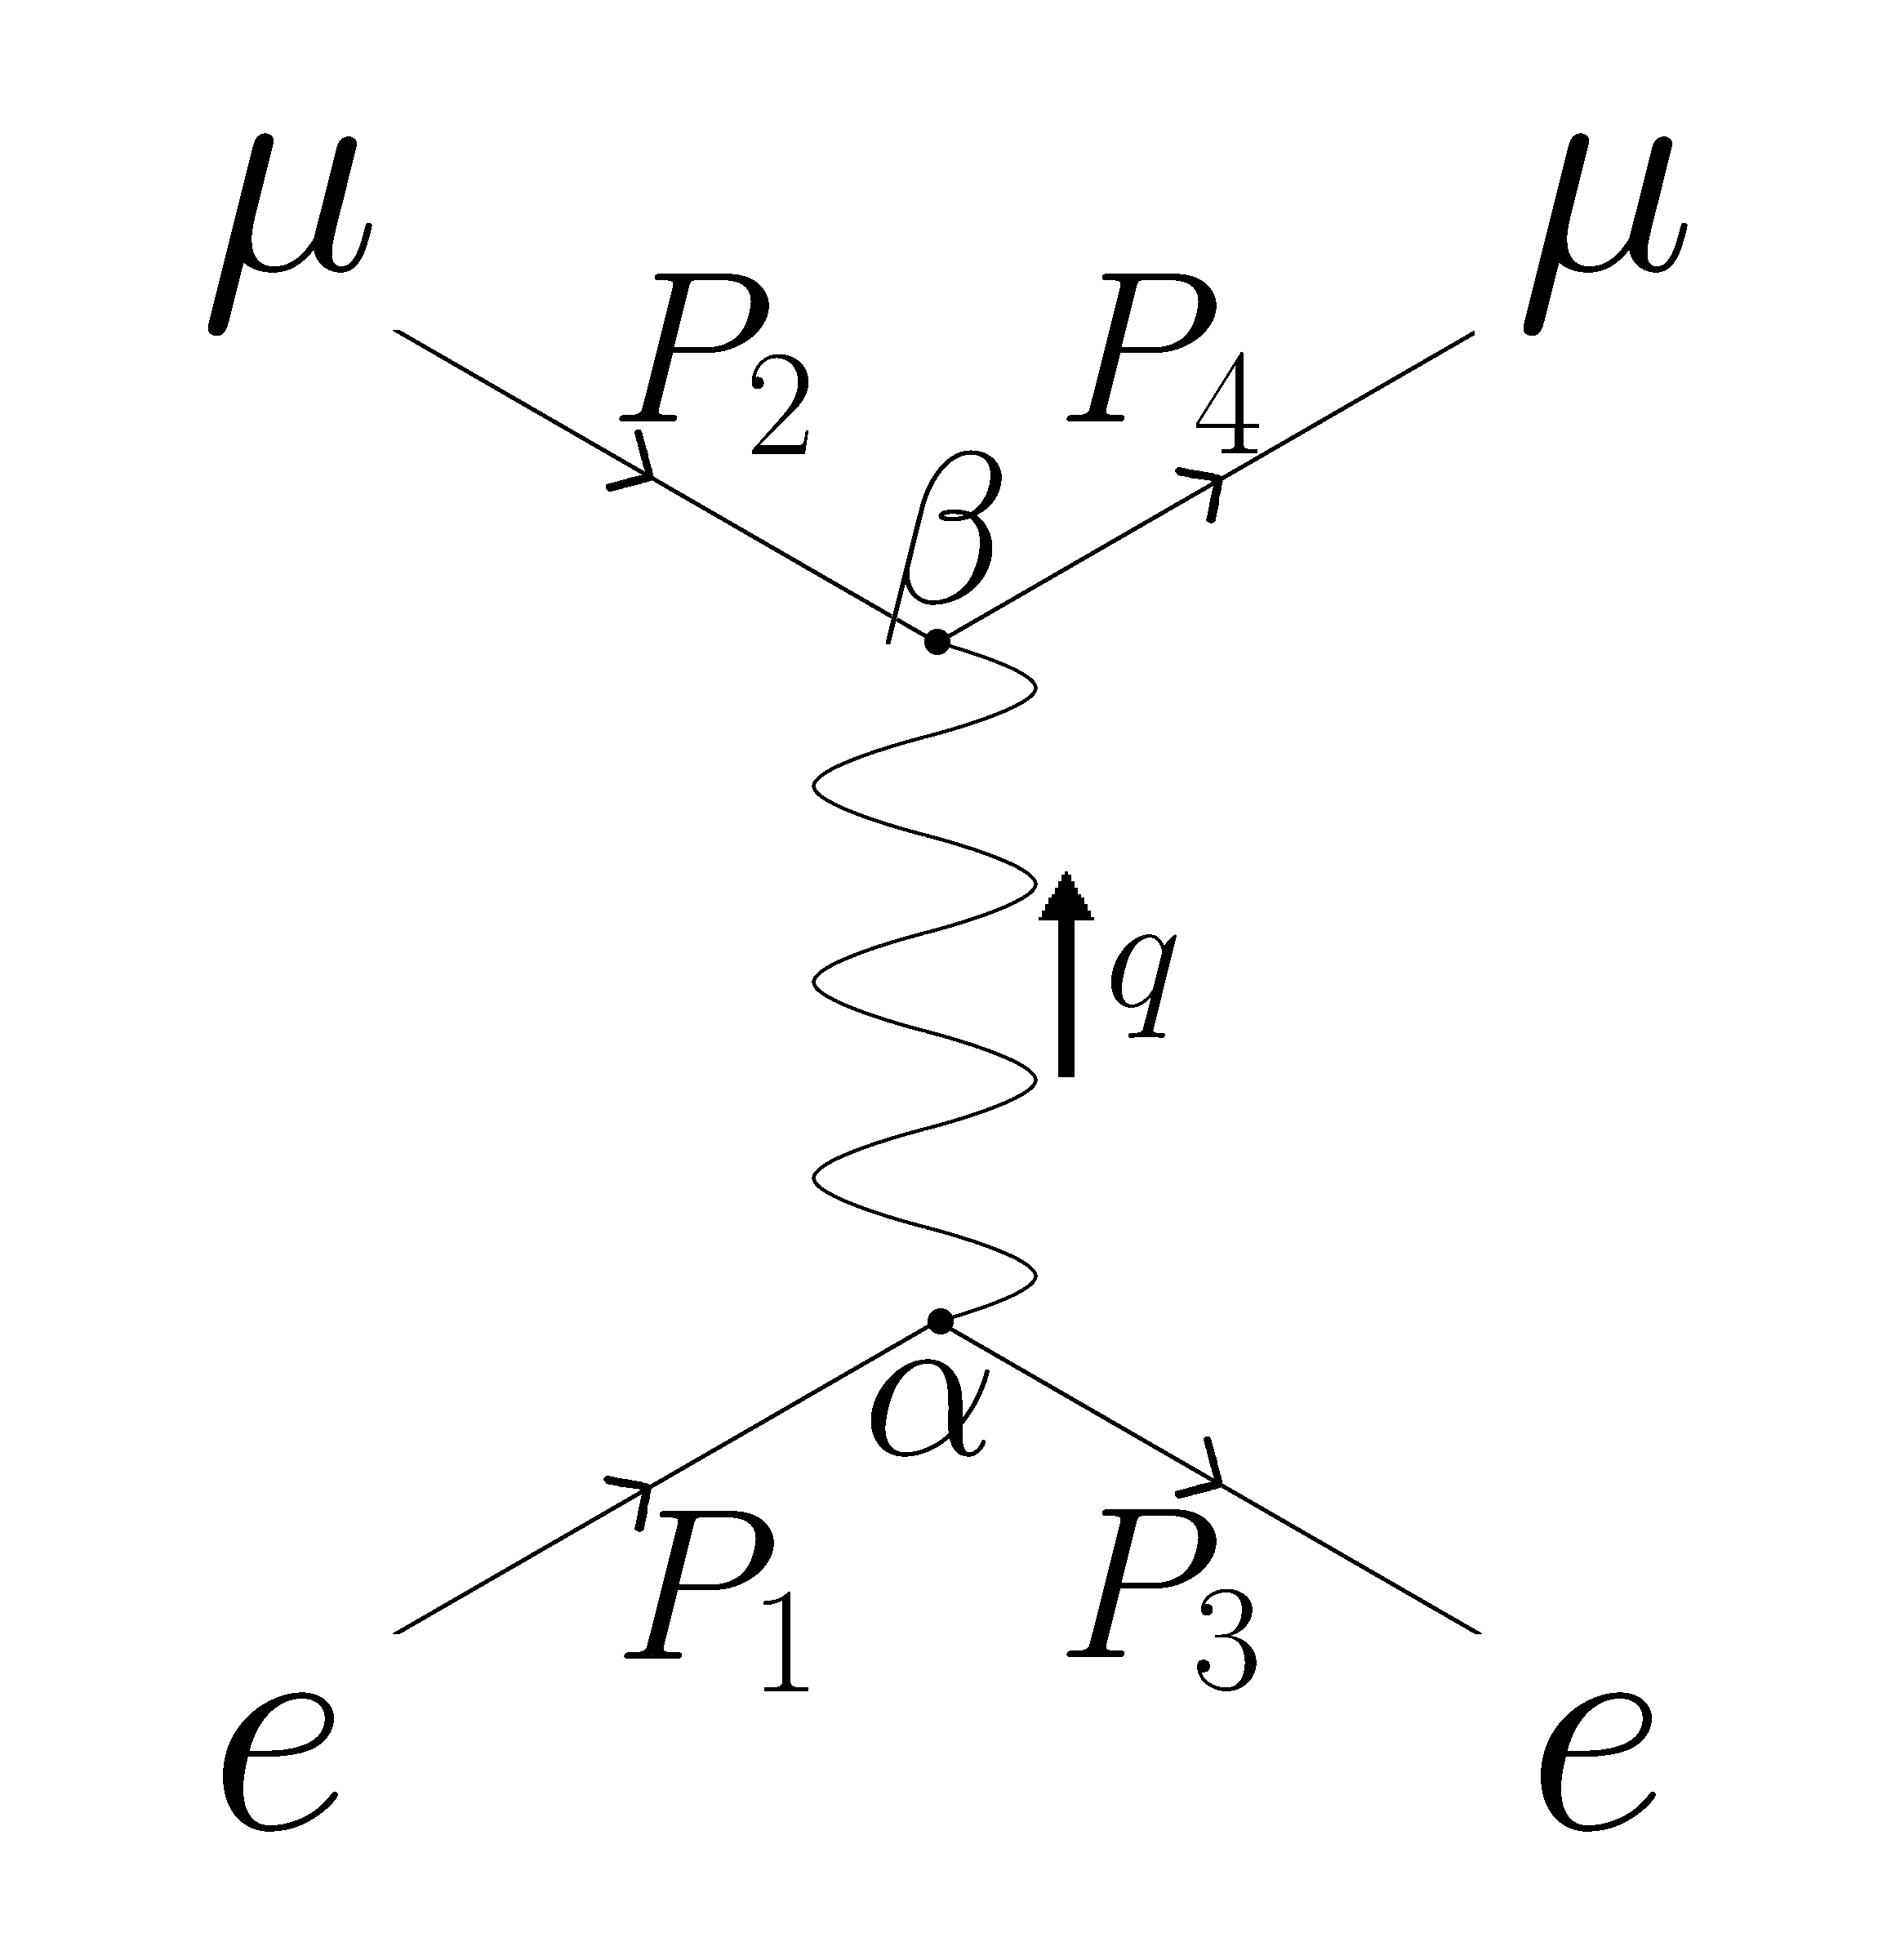
\includegraphics[width=0.5\textwidth]{Figures/MottFeynman} 
  \caption{Feynman diagram for electron-muon scattering. $P_1$ and $P_2$ are the incoming four-momenta for the electron and muon and $P_3$ and $P_4$ are the outgoing four-momenta. $Q$ represents the four-momentum carried by the virtual photon.}
  \label{fig:mottFeynmanSupplemental}
\end{figure}

The fermion flow is the path which goes along the directions of the arrows. For example, the first fermion flow which is observed is the muon flow: a muon enters from the left, there is an interaction at the propagator vertex $\beta$, and a muon exits from the right. Each muon contributes its spinor, and the outgoing muon and incoming muon are adjoints of one another (i.e. if the spinor of $P_2$ is $U(P_2)$ then the spinor of $P_4$ is $\bar{U}(P_4)$). The propagator vertex contributes a factor of $-ieQ_\mu\gamma^\beta$. Since matrices compound right-to-left, it is necessary to start at the end of the fermion flow and work backwards. Then
\begin{figure}
  \centering
    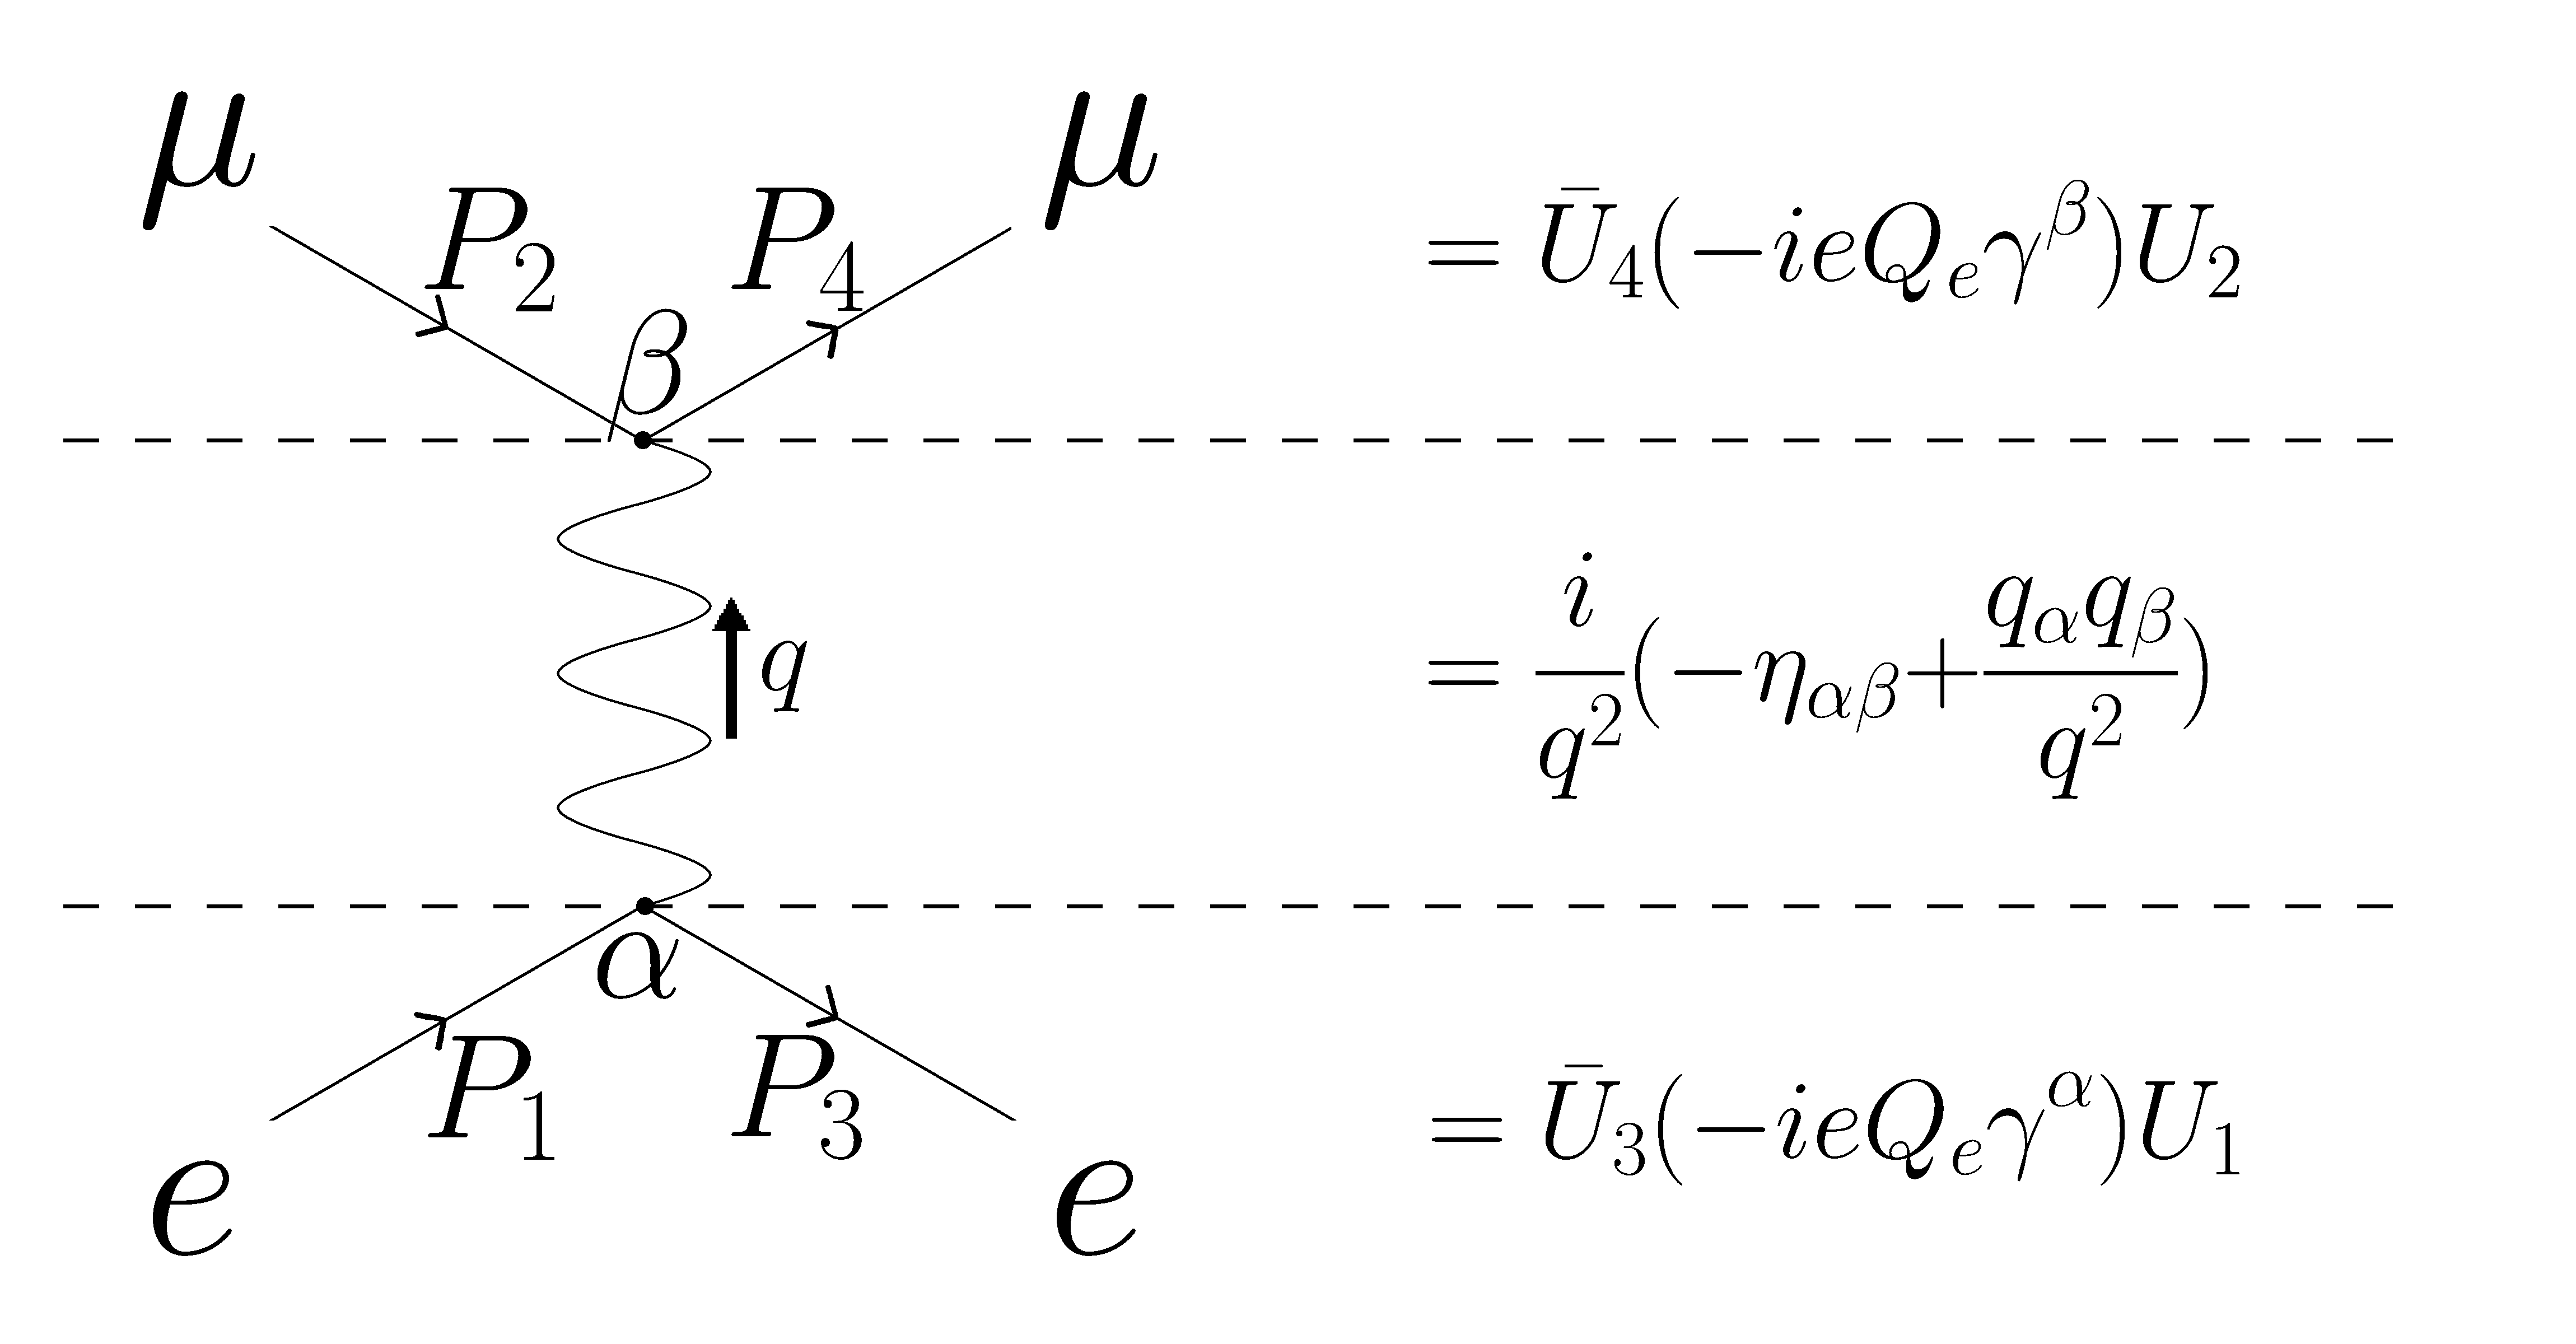
\includegraphics[width=\textwidth]{Figures/MottFeynmanMath} 
  \caption{Mathematical interpretation the three branches of the Feynman diagram in Figure \ref{fig:mottFeynmanSupplemental}. The top part is the muon flow, the middle is the virtual photon, and the bottom is the electron flow.}
  \label{fig:mottFeynmanMath}
\end{figure}
Then the scattering amplitude is
\begin{equation} \label{eqn:mottFeynmanScatteringAmplitude}
i\mathcal{M}=\bar{U}_4(-ieQ_\mu\gamma^\beta)U_2\cdot\frac{i}{q^2}(-\eta_{\alpha\beta}+\frac{q_\alpha q_\beta}{q^2})\cdot\bar{U}_3(-ieQ_e\gamma^\alpha)U_1.
\end{equation}